\documentclass[simplex.tex]{subfiles}
% NO NEED TO INPUT PREAMBLES HERE
% packages are inherited; you can compile this on its own
%\usepackage{caption}
%\usepackage{subcaption}

\begin{document}
\subsection{Law of Large Graphs}
We note that low-rank methods can often be more easily interpreted.
By representing a low-rank matrix in terms of the latent position, where each vertex is represented as a vector in $\Re^d$ and the entries of the matrix are given by the inner products of these vectors, one can analyze and visualize the geometry of these vectors in order to interpret how each vertex is behaving in the context of the larger graph. 
Now we take the CoRR dataset experiment as an example and consider the same sample of size $M=5$ based on the Desikan atlas. Our estimator $\hat{P}$ is based on the estimated latent positions $\hat{X} \in \mathbb{R}^{N\times d}$, where $N=70$ is the number of vertices and $d=11$ is the dimension selected by the Zhu and Ghodsi's method. 
We color the brain using the first 5 dimensions of $\hat{X}$ as in Fig.~\ref{fig:eigenvector_brain}. 
From the figures, we can see the embeddings have its own neuro-meaning, for example there is a clear distinction of the left and right hemisphere as conveyed in the second dimension. Also, the first dimension provides an average level of the entire brain. We are still exploring the interpretation other dimensions are providing.


\begin{figure}	
\centering
\begin{subfigure}[t]{0.6\textwidth}
\caption{1st dimension}
\vspace*{-15pt}
\begin{center}
  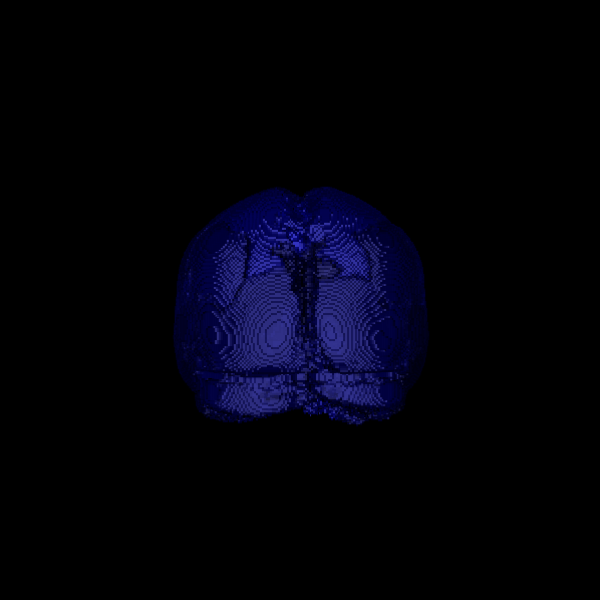
\includegraphics[height=.33\linewidth]{../../figs/desikan1a.png}\hspace{-20pt}
  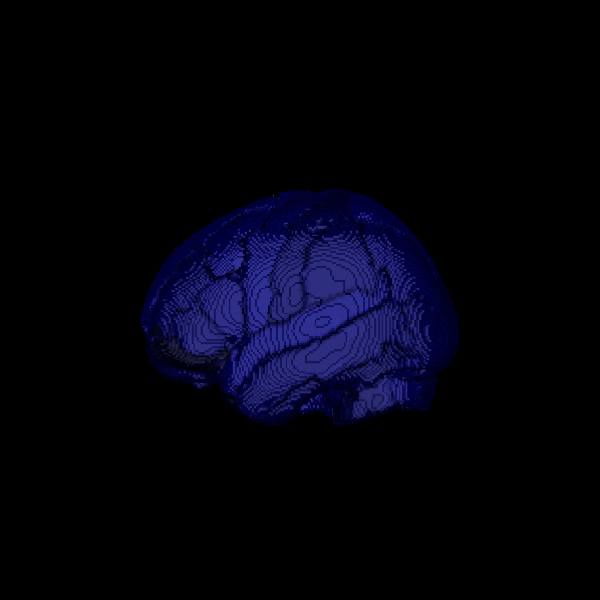
\includegraphics[height=.33\linewidth]{../../figs/desikan1b.png}\hspace{-20pt}
  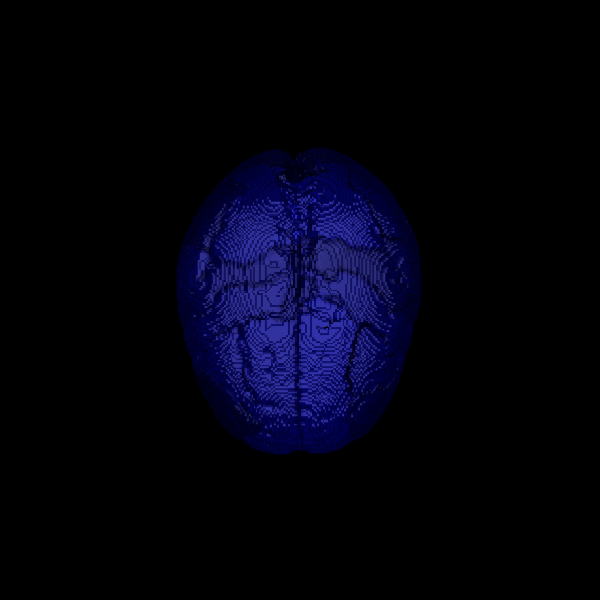
\includegraphics[height=.33\linewidth]{../../figs/desikan1c.png}
\end{center}
\end{subfigure}\\
\vspace*{5pt}
\begin{subfigure}[t]{0.6\textwidth}
\caption{2nd dimension}
\vspace*{-15pt}
\begin{center}
  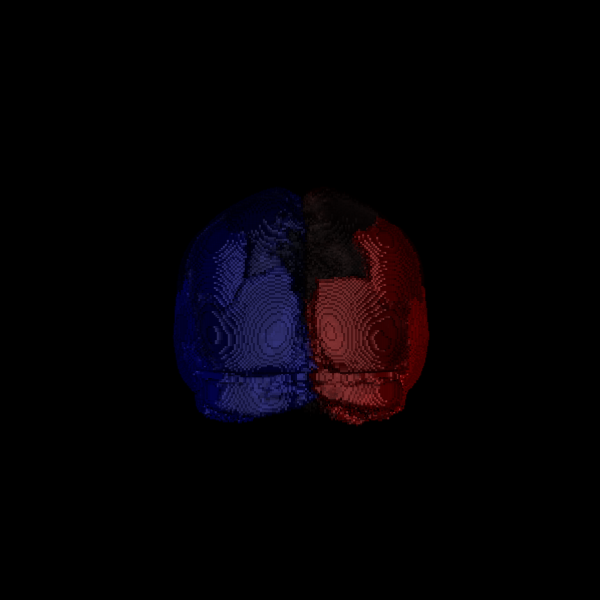
\includegraphics[height=.33\linewidth]{../../figs/desikan2a.png}\hspace{-20pt}
  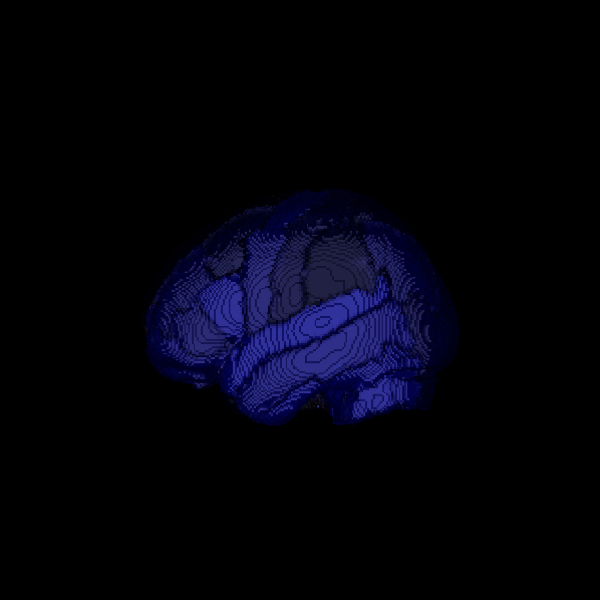
\includegraphics[height=.33\linewidth]{../../figs/desikan2b.png}\hspace{-20pt}
  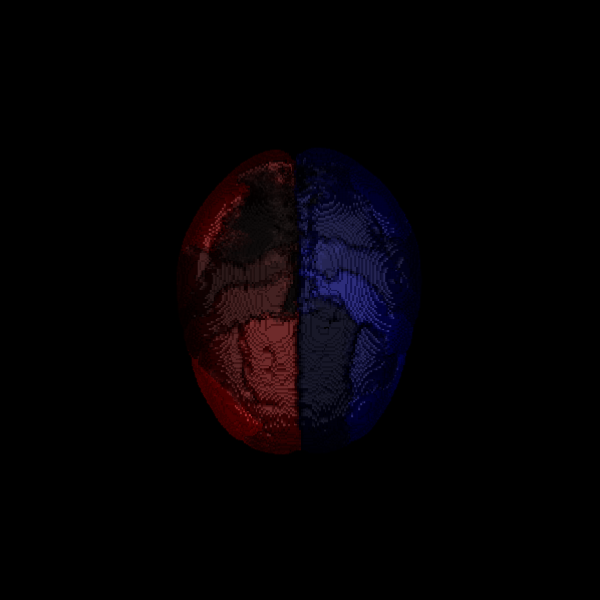
\includegraphics[height=.33\linewidth]{../../figs/desikan2c.png}
\end{center}
\end{subfigure}\\
\vspace*{5pt}
\begin{subfigure}[t]{0.6\textwidth}
\caption{3rd dimension}
\vspace*{-15pt}
\begin{center}
  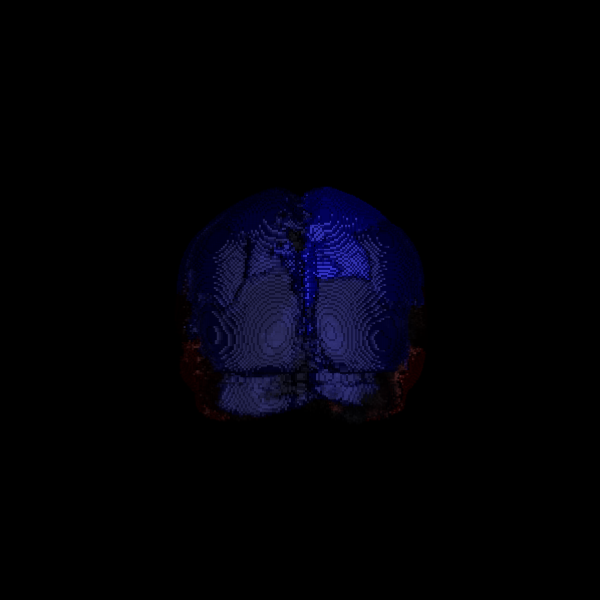
\includegraphics[height=.33\linewidth]{../../figs/desikan3a.png}\hspace{-20pt}
  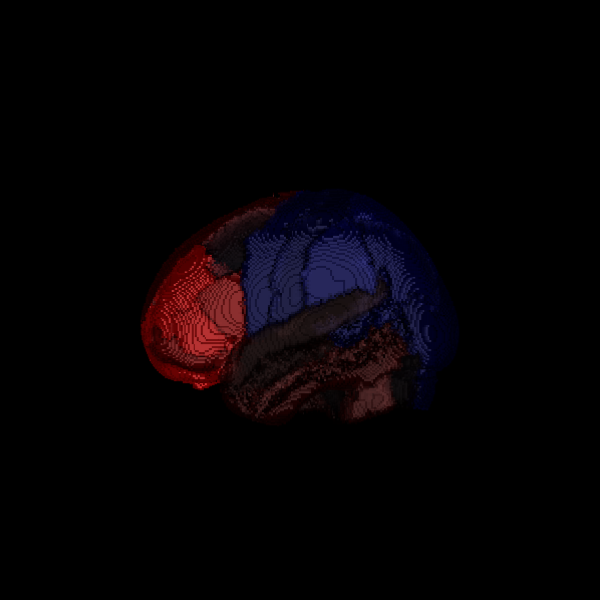
\includegraphics[height=.33\linewidth]{../../figs/desikan3b.png}\hspace{-20pt}
  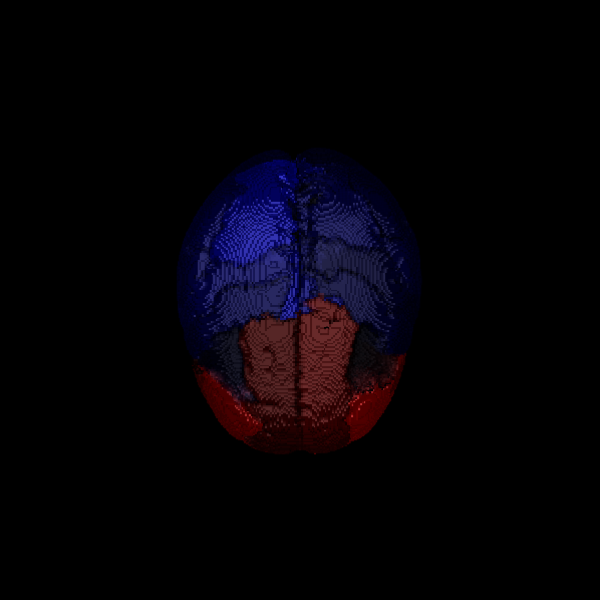
\includegraphics[height=.33\linewidth]{../../figs/desikan3c.png}
\end{center}
\end{subfigure}\\
\vspace*{5pt}
\begin{subfigure}[t]{0.6\textwidth}
\caption{4th dimension}
\vspace*{-15pt}
\begin{center}
  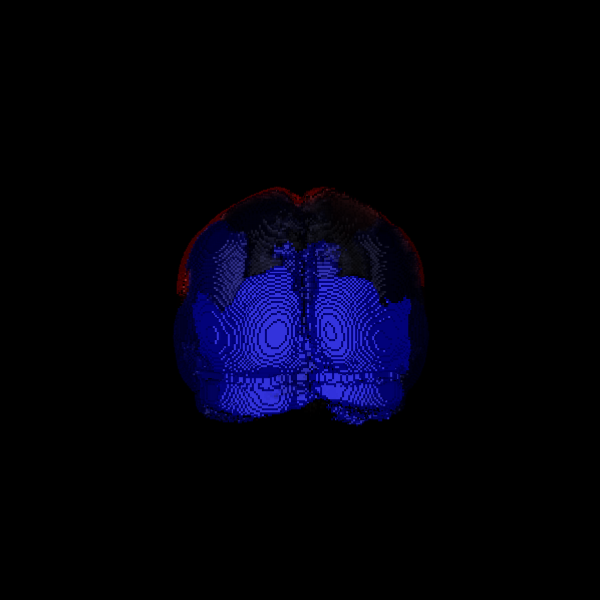
\includegraphics[height=.33\linewidth]{../../figs/desikan4a.png}\hspace{-20pt}
  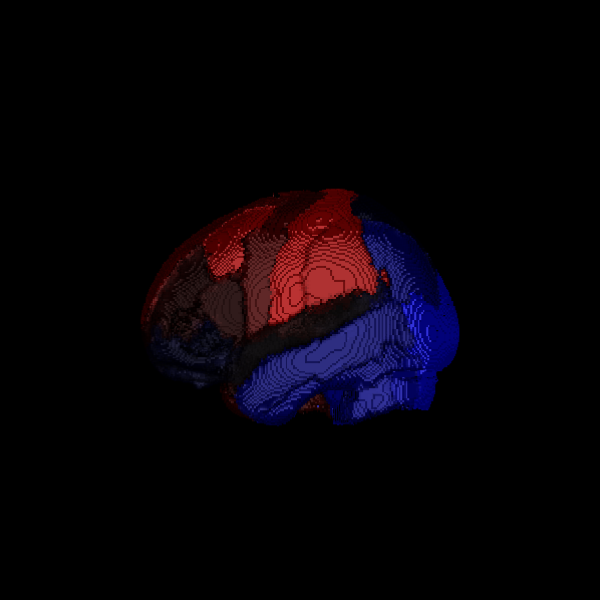
\includegraphics[height=.33\linewidth]{../../figs/desikan4b.png}\hspace{-20pt}
  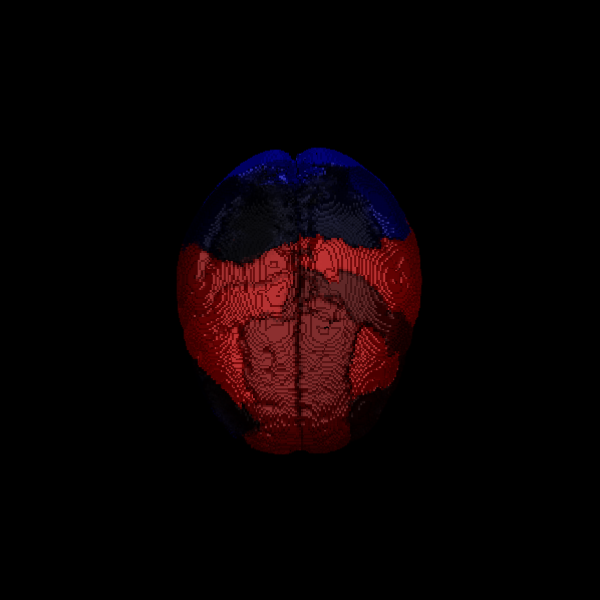
\includegraphics[height=.33\linewidth]{../../figs/desikan4c.png}
\end{center}
\end{subfigure}\\
\vspace*{5pt}
\begin{subfigure}[t]{0.6\textwidth}
\caption{5th dimension}
\vspace*{-15pt}
\begin{center}
  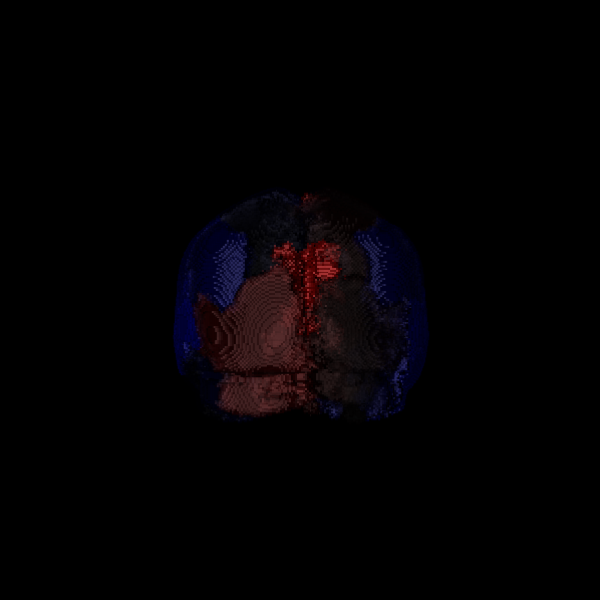
\includegraphics[height=.33\linewidth]{../../figs/desikan5a.png}\hspace{-20pt}
  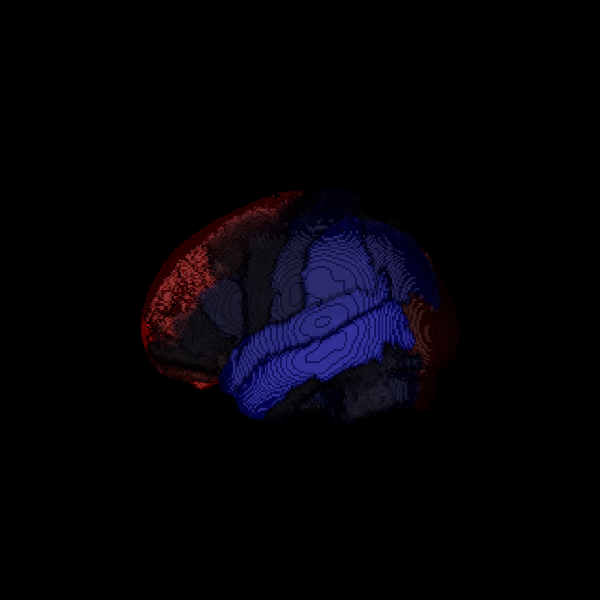
\includegraphics[height=.33\linewidth]{../../figs/desikan5b.png}\hspace{-20pt}
  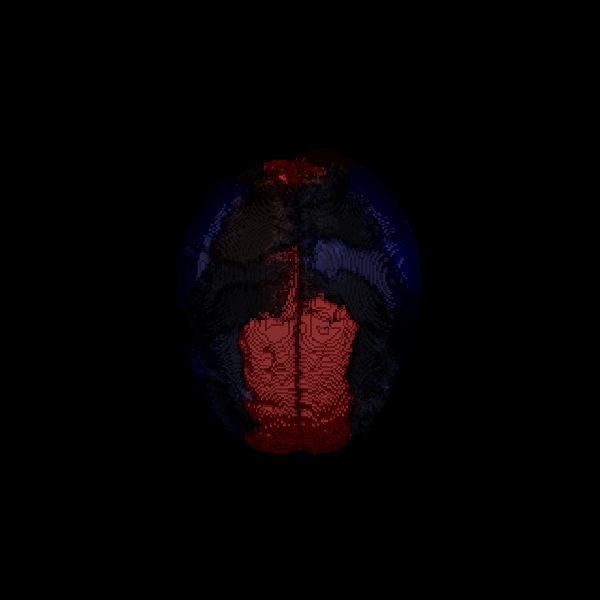
\includegraphics[height=.33\linewidth]{../../figs/desikan5c.png}
\end{center}
\end{subfigure}\\
\caption{\textbf{Brain plots colored by the first 5 dimensions of $\hat{X}$ for the Desikan atlas respectively.} We plot the brain using the first 5 dimension of $\hat{X}$ . From the figures, we can see the embeddings have its own neuro-meaning, for example there is a clear distinction of the left and right hemisphere as conveyed in the second dimension. Also, the first dimension provides an average level of the entire brain.}
\label{fig:eigenvector_brain}
\end{figure}

%
\clearpage
\end{document}
